\begin{tabular}{p{0.5\textwidth} p{0.5\textwidth}}
  \tablesubsection{Work Done by a Constant Force}
   & \\%adds spacing stuff
\end{tabular}

%commands for positioning the triangle
\newcommand{\triht}{5cm}
\newcommand{\triwd}{7cm}

\newcommand{\dispht}{1cm}
\newcommand{\dispwd}{10cm}

% http://tex.stackexchange.com/questions/166958/draw-with-tikz-a-pythagorean-triangle-with-the-squares-of-its-sides-and-labels
% http://tex.stackexchange.com/questions/96459/automatically-draw-and-labels-angles-of-a-triangle-in-tikz

\begin{center}
  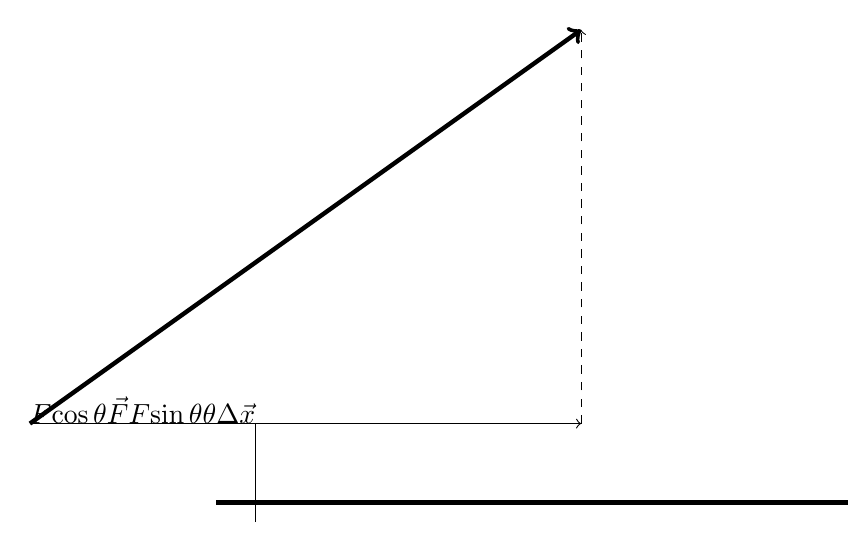
\begin{tikzpicture}%[thick]
    \coordinate (A) at (0,0);
    \coordinate (B) at (0+\triwd,0);
    \coordinate (C) at (0+\triwd,0+\triht);

    \draw [->] (A)--(B);
    \draw [dashed, ->] (B)--(C);
    \draw [ultra thick, ->] (A)--(C);

    \tkzLabelSegment[below=2pt](A,B){${F}{\cos\theta}$}
    \tkzLabelSegment[left=2pt](A,C){$\vec{F}$}
    \tkzLabelSegment[above right=2pt](B,C){$\cancel{{F}{\sin\theta}}$}

    % \tkzMarkRightAngle[fill=orange,size=0.5,opacity=.4](A,B,C)% square angle here
    % \tkzLabelAngle[pos = 0.35](A,B,C){$\gamma$}

    \tkzMarkAngle[fill= blue,size=1.5cm,opacity=.4](B,A,C)
    \tkzLabelAngle[pos = 0.75](B,A,C){$\theta$}

    % \tkzMarkAngle[fill= orange,size=0.7cm,opacity=.4](A,C,B)
    % \tkzLabelAngle[pos = 0.5](A,C,B){$\beta$}

    \coordinate (Xi) at (0,-\dispht);
    \coordinate (Xf) at (\dispwd,-\dispht);

    \coordinate (Xi_bar1) at (0,-\dispht-0.25cm);
    \coordinate (Xf_bar1) at (\dispwd,-\dispht-0.25cm);
    \coordinate (Xi_bar2) at (0,0);
    \coordinate (Xf_bar2) at (\dispwd,0);


    \draw [ultra thick, ->] (Xi)--(Xf);
    \tkzLabelSegment[below=2pt](Xi,Xf){$\Delta \vec{x}$}
    % \draw [o] (0,-\dispht);

    \draw (Xi_bar1)--(Xi_bar2);
    \draw (Xf_bar1)--(Xf_bar2);

  \end{tikzpicture}
\end{center}

A constant force $\vec{F}$ exerted at an angle $\theta$ with respect to the displacement, $\Delta\vec{x}$, performs work \(\displaystyle W = ({F}{\cos\theta}){\Delta x}\).
%%% Local Variables:
%%% mode: latex
%%% TeX-master: "../main"
%%% End:
